\documentclass[12pt,a4paper]{article}

% --- Packages ---
\usepackage[utf8]{inputenc}
\usepackage[T1]{fontenc}
\usepackage{lmodern}
\usepackage[english]{babel}
\usepackage{geometry}
\usepackage{amsmath,amssymb}
\usepackage{graphicx}
\usepackage{booktabs}
\usepackage{tabularx}
\usepackage{listings}
\usepackage{xcolor}
\usepackage{fancyhdr}
\usepackage[many]{tcolorbox}
\usepackage{microtype}
\usepackage{pgfplots}
\pgfplotsset{compat=1.18}
\usepackage{hyperref}

% --- Page Setup ---
\geometry{
    top=2.5cm,
    bottom=2.5cm,
    left=2.5cm,
    right=2.5cm
}

% --- Custom Colors ---
\definecolor{primary}{RGB}{18, 52, 86}
\definecolor{secondary}{RGB}{41, 128, 185}
\definecolor{accent}{RGB}{231, 76, 60}
\definecolor{codebg}{RGB}{247, 249, 250}
\definecolor{codeframe}{RGB}{209, 213, 219}
\definecolor{codegreen}{RGB}{39, 136, 60}
\definecolor{codepurple}{RGB}{137, 89, 168}
\definecolor{codegray}{RGB}{108, 117, 125}
\definecolor{termbg}{RGB}{0, 0, 0}
\definecolor{termfg}{RGB}{255, 255, 255}
\definecolor{termgreen}{RGB}{80, 250, 123}
\definecolor{termred}{RGB}{255, 85, 85}
\definecolor{termyellow}{RGB}{241, 250, 140}
\definecolor{termcyan}{RGB}{139, 233, 253}

% --- Romanian Character Literate for Listings ---
\lstset{
    extendedchars=true,
    literate=%
        {ă}{{\u{a}}}1
        {Ă}{{\u{A}}}1
        {â}{{\^a}}1
        {Â}{{\^A}}1
        {î}{{\^\i}}1
        {Î}{{\^I}}1
        {ș}{{\c{s}}}1
        {Ș}{{\c{S}}}1
        {ț}{{\c{t}}}1
        {Ț}{{\c{T}}}1
        {ş}{{\c{s}}}1
        {Ş}{{\c{S}}}1
        {ţ}{{\c{t}}}1
        {Ţ}{{\c{T}}}1
}

% --- Listings Setup ---
\lstset{
    language=[Sharp]C,
    backgroundcolor=\color{codebg},
    basicstyle=\small\ttfamily,
    keywordstyle=\color{secondary}\bfseries,
    stringstyle=\color{codegreen},
    commentstyle=\color{codegray}\itshape,
    numberstyle=\tiny\color{codegray},
    numbers=left,
    stepnumber=1,
    numbersep=10pt,
    tabsize=4,
    showspaces=false,
    showstringspaces=false,
    breaklines=true,
    breakatwhitespace=true,
    frame=single,
    rulecolor=\color{codeframe},
    captionpos=b,
    keepspaces=true
}

\tcbuselibrary{listings,skins}

% --- Terminal Box Setup ---
\newtcblisting{terminalwindow}[1][]{%
    enhanced,
    colback=black,
    colframe=black,
    arc=2.5mm,
    boxrule=1pt,
    title={\textcolor{termred}{$\bullet$}\;\textcolor{termyellow}{$\bullet$}\;\textcolor{termgreen}{$\bullet$}\quad \textsf{\bfseries Console Terminal Session}},
    fonttitle=\small\sffamily\bfseries,
    coltitle=white,
    attach boxed title to top left={yshift=-2mm, xshift=4mm},
    boxed title style={colback=gray!15!black, arc=1.5mm, boxrule=0.5pt},
    listing only,
    listing options={
        backgroundcolor=\color{black},
        basicstyle=\small\ttfamily\color{white},
        frame=none,
        numbers=none,
        breaklines=true,
        tabsize=4,
        showspaces=false,
        showstringspaces=false,
        extendedchars=true,
        literate=%
            {ă}{{\u{a}}}1
            {Ă}{{\u{A}}}1
            {â}{{\^a}}1
            {Â}{{\^A}}1
            {î}{{\^\i}}1
            {Î}{{\^I}}1
            {ș}{{\c{s}}}1
            {Ș}{{\c{S}}}1
            {ț}{{\c{t}}}1
            {Ț}{{\c{T}}}1
            {ş}{{\c{s}}}1
            {Ş}{{\c{S}}}1
            {ţ}{{\c{t}}}1
            {Ţ}{{\c{T}}}1
    },
    #1
}

% --- Hyperlink Setup ---
\hypersetup{
    colorlinks=true,
    linkcolor=primary,
    citecolor=secondary,
    urlcolor=secondary
}

% --- Headers & Footers ---
\pagestyle{fancy}
\fancyhf{}
\setlength{\headheight}{15pt}
\addtolength{\topmargin}{-3pt}
\fancyhead[L]{\small\textsf{Laboratory Work No. 1 --- Network Programming}}
\fancyhead[R]{\small\textsf{Vitalie Vasilean}}
\fancyfoot[C]{\thepage}
\renewcommand{\headrulewidth}{0.4pt}
\renewcommand{\footrulewidth}{0pt}

% --- Macros ---
\newcommand{\studentgroup}{FAF-241}

\begin{document}

% =========================================================================
% TITLE PAGE
% =========================================================================
\begin{titlepage}
    \centering
    {\large \textbf{TECHNICAL UNIVERSITY OF MOLDOVA}}\\[0.2cm]
    {\large Faculty of Computers, Informatics and Microelectronics}\\[0.2cm]
    {\large Department of Software Engineering and Automatics}\\[0.8cm]

    
\includegraphics[width=3.5cm]{figures/utm_logo.png}\\[1.2cm]

    {\Large \textbf{LABORATORY WORK NO. 1}}\\[0.4cm]
    {\LARGE \textbf{Concurrency in Practice: Multithreading, Shared State, and I/O Performance Analysis}}\\[0.4cm]
    {\large Course: Network Programming}\\[2.5cm]

    \begin{minipage}{0.45\textwidth}
        \flushleft
        \textbf{Author:}\\
        Vitalie \textsc{Vasilean}\\
        Student of group: \studentgroup
    \end{minipage}
    \hfill
    \begin{minipage}{0.45\textwidth}
        \flushright
        \textbf{Verified by:}\\
        Lecturer / Supervisor\\
        Ernest B\^{\i}tca
    \end{minipage}

    \vfill
    {\large Chi\c{s}in\u{a}u --- 2026}
\end{titlepage}

\newpage
\tableofcontents
\newpage

% =========================================================================
% 1. INTRODUCTION AND OBJECTIVES
% =========================================================================
\section{Introduction and Laboratory Objectives}

Concurrent and parallel execution is fundamental to network programming and high-performance distributed systems. Understanding how modern operating system threads interact with multi-core processor architectures, memory hierarchies, and storage subsystems allows software engineers to design scalable services that avoid synchronization bottlenecks, data corruption, and resource starvation.

The primary objectives of this laboratory work are:
\begin{enumerate}
    \item \textbf{Measure Thread Scalability:} Empirically evaluate how thread scaling ($p \in \{1, 2, 4, 8, 16, 32, 64\}$) affects execution time, parallel speed-up, and memory overhead when processing large-scale numeric workloads ($50\,000\,000$ integers).
    \item \textbf{Characterize CPU-Bound vs. I/O-Bound Regimes:} Differentiate workload regimes based on whether performance is constrained by arithmetic and parsing throughput or by storage bus bandwidth and latency.
    \item \textbf{Analyze Shared State and Synchronization Costs:} Observe race conditions resulting from unsynchronized access to shared counters, quantify the synchronization overhead of mutual exclusion locks, and demonstrate lock-free per-thread accumulation.
    \item \textbf{Evaluate Producer-Consumer Architectures:} Implement and benchmark a decoupled producer-consumer pipeline with bounded queues, examining the trade-offs of queue capacities, batch sizes, and worker thread contention.
    \item \textbf{Assess I/O Scalability on Slow Storage:} Investigate the behavior of multi-threaded I/O operations against removable flash media while circumventing operating system page caching mechanisms.
\end{enumerate}

% =========================================================================
% 2. HARDWARE AND ENVIRONMENT SPECIFICATIONS
% =========================================================================
\section{Hardware and Environment Specifications}

Per laboratory requirements, all experimental evaluations were conducted on a dedicated physical host. The complete hardware specifications and runtime environment details are documented in Table~\ref{tab:hardware_specs}.

\begin{table}[htbp]
\centering
\caption{System Hardware and Runtime Environment Specifications}
\label{tab:hardware_specs}
\small
\begin{tabularx}{\textwidth}{lX}
\toprule
\textbf{Component} & \textbf{Specification / Value} \\
\midrule
\textbf{Host Device} & Lenovo IdeaPad Slim (Model: 83GH, ARM64 Platform) \\
\textbf{Processor (CPU)} & Qualcomm Snapdragon(R) X Plus - X1P42100 \\
\textbf{CPU Architecture} & ARMv8 (64-bit), Qualcomm(R) Oryon(TM) Architecture \\
\textbf{Physical Cores} & 8 Physical Cores \\
\textbf{Logical Processors} & 8 Logical Processors (1 thread per core, SMT disabled) \\
\textbf{Max Clock Speed} & 3.24 GHz (3244 MHz) \\
\textbf{System Memory (RAM)} & 16.0 GB LPDDR5X (Configured Clock Speed: 8448 MT/s) \\
\textbf{Primary Storage (Disk)} & Samsung PM9B1 NVMe SSD (MZAL8512HDLU-00BL2, 512 GB, PCIe 4.0 x4, NTFS) \\
\textbf{Removable Storage (USB/SD)} & Apacer USB Flash Drive / SDHC Storage (3.64 GB usable, FAT32, USB 2.0 interface) \\
\textbf{Operating System} & Microsoft Windows 11 Home (Build 26200, 64-bit ARM) \\
\textbf{Language \& Compiler} & C\# 13.0 \\
\textbf{Runtime \& SDK} & .NET 10.0.12 Runtime / .NET SDK 10.0.401 (\texttt{win-arm64}) \\
\bottomrule
\end{tabularx}
\end{table}

\subsection{Architectural Implications}
The Qualcomm Snapdragon X Plus platform features 8 dedicated high-performance Oryon CPU cores. Unlike conventional x86 processors that implement Simultaneous Multithreading (Intel Hyper-Threading or AMD SMT), this ARM64 SoC provides an exact 1:1 mapping between physical cores and logical processors ($P = L = 8$). Consequently:
\begin{itemize}
    \item Parallel workloads should exhibit near-linear speed-up up to 8 threads, provided synchronization and memory bus contention remain negligible.
    \item Beyond 8 threads (e.g., 16, 32, 64 threads), the OS thread scheduler is forced to perform preemptive time-slicing and context switching, incurring CPU cache invalidation and thread migration penalties.
    \item The 8448 MT/s LPDDR5X memory subsystem provides ultra-high memory bandwidth, minimizing memory access bottlenecks during in-memory processing.
\end{itemize}

% =========================================================================
% 3. THEORETICAL BACKGROUND
% =========================================================================
\section{Theoretical Background}

\subsection{Concurrency vs. Parallelism}
\textbf{Concurrency} is the composition of independently executing processes or computations. A system is concurrent if it can handle multiple tasks by interleaving their execution over time. In contrast, \textbf{Parallelism} is the simultaneous physical execution of multiple computations across separate processor cores. 
On an 8-core machine, true parallelism occurs when up to 8 active OS threads execute concurrently on distinct hardware cores.

\subsection{Amdahl's Law and Scaling Bottlenecks}
Amdahl's Law characterizes the theoretical upper bound of speed-up achievable by parallelizing a workload across $p$ processing units:
\begin{equation}
    S(p) = \frac{1}{(1 - f) + \frac{f}{p}}
\end{equation}
where $f$ represents the parallelizable proportion of the program, and $(1 - f)$ is the strictly serial fraction (such as initial file opening, work splitting, queue initialization, or final result aggregation). Even with an infinite number of threads ($p \to \infty$), the speed-up is capped at $S_{\max} = \frac{1}{1 - f}$. In practice, scaling beyond physical core capacity introduces non-zero scheduling overheads $\mathcal{O}_{\text{overhead}}(p)$, causing speed-up to decline.

\subsection{Shared State, Race Conditions, and Synchronization}
A \textbf{data race} occurs when two or more threads access a shared memory location concurrently, at least one access is a write, and no synchronization mechanisms coordinate the operations. 
In high-level languages like C\#, an expression such as \texttt{counter++} is not an atomic operation. Under the hood, it compiles to a three-step instruction sequence:
\begin{enumerate}
    \item \textbf{Load:} Read the current counter value from memory/L1 cache into a CPU register ($R_1 \leftarrow [\text{counter}]$).
    \item \textbf{Modify:} Increment the value within the register ($R_1 \leftarrow R_1 + 1$).
    \item \textbf{Store:} Write the updated register value back to memory ($[\text{counter}] \leftarrow R_1$).
\end{enumerate}
When multiple threads execute this sequence without synchronization, interleaving causes one thread to overwrite another's update with an outdated register value, leading to lost updates.

\subsubsection{Synchronization Strategies}
\begin{itemize}
    \item \textbf{Mutual Exclusion Locks (\texttt{lock} / \texttt{Monitor}):} Enforces serialization of the critical section. While mathematically correct, it introduces lock acquisition overhead, kernel context switching when threads block, and severe cache line bouncing across CPU cores.
    \item \textbf{Thread-Local Aggregation:} Eliminates shared memory contention entirely by providing each thread with private counters. After thread termination, a single-threaded reduction sums the private counters into a final total in $\mathcal{O}(p)$ time.
\end{itemize}

\subsection{Producer-Consumer Pipeline and Bounded Channels}
The Producer-Consumer pattern decouples data acquisition (I/O reading) from data processing (parsing and sign evaluation). 
A bounded queue of capacity $C$ acts as an elastic buffer:
\begin{itemize}
    \item When the buffer reaches $C$ items, the producer blocks, preventing unbounded memory growth.
    \item When the buffer is empty, consumer threads block until new batches are available.
    \item Batching items (e.g., 10\,000 lines per batch) amortizes lock and signaling costs across many elements, drastically decreasing queuing overhead.
\end{itemize}

% =========================================================================
% 4. SYSTEM IMPLEMENTATION
% =========================================================================
\section{System Architecture and Implementation}

The application is implemented as a unified command-line tool in C\# targeting .NET 10. Every task and configuration parameter is dynamically selected via CLI arguments.

\subsection{Dataset Generation}
A utility command generates \texttt{numbers.txt} containing $50\,000\,000$ uniformly distributed integers in the range $[-1\,000\,000, 1\,000\,000]$, written one per line. For Task 2, the dataset is evenly split in sequential order into 8 separate files (\texttt{numbers\_part0.txt} through \texttt{numbers\_part7.txt}), each containing exactly $6\,250\,000$ integers.
A global verification invariant guarantees that for every execution:
\begin{equation}
    \text{Count}_{\text{neg}} + \text{Count}_{\text{pos}} + \text{Count}_{\text{zero}} = 50\,000\,000
\end{equation}

\subsection{Task 1a: File Partitioning with Parallel Threads}
To parallelize the reading of a single large file without duplicate or skipped records:
\begin{enumerate}
    \item The file size in bytes $S$ is divided into $N$ equal chunks of nominal size $B = \lfloor S / N \rfloor$.
    \item For thread $i \in \{0, \dots, N-1\}$, the byte offset starts at $i \cdot B$ and ends at $(i+1) \cdot B$ (with the last thread extending to EOF).
    \item \textbf{Boundary Handling:} If $i > 0$, thread $i$ seeks to $i \cdot B$, discards the partial line up to the first newline character, and begins reading from the subsequent complete line.
    \item Meanwhile, thread $i - 1$ continues reading past its nominal end boundary $(i \cdot B)$ until it consumes the first complete newline, cleanly handing off the stream without overlaps.
\end{enumerate}

\subsection{Task 1b: Three Strategies for Sign Counting}
The complete dataset is loaded into a contiguous 32-bit integer array \texttt{int[50\_000\_000]}. With 8 worker threads matching the hardware's 8 logical cores, numbers are processed under three synchronization models:
\begin{enumerate}
    \item \textbf{Version 1 (Unsynchronized):} All threads increment shared fields \texttt{pos}, \texttt{neg}, and \texttt{zero} directly. Demonstrates race conditions and lost updates.
    \item \textbf{Version 2 (Lock-Protected):} Updates are enclosed in a \texttt{lock(syncRoot)} critical section. Guarantees mathematical correctness at the expense of high lock contention.
    \item \textbf{Version 3 (Thread-Local Accumulators):} Each thread increments private local variables. Upon thread completion, local results are combined using a lock-free reduction.
\end{enumerate}

\subsection{Task 1c: Bounded Producer-Consumer Pipeline}
A dedicated reader thread reads lines from \texttt{numbers.txt}, groups them into batches of $10\,000$ lines, and enqueues them into a bounded queue with a maximum capacity of 100 batches. Worker threads ($1, 2, 4, 8, 16, 32, 64$) dequeue batches, parse numbers, and aggregate counters locally.

\subsection{Task 2: Multi-File Processing on Slow Storage}
The 8 chunk files are located on an external USB flash drive / removable storage. To prevent the operating system from serving file requests from RAM (standby cache / dirty page cache), the drive is unmounted/remounted prior to execution. Each file is ingested in a single read call into a contiguous byte buffer, parsed in memory, and counted across 1, 2, and 4 worker threads.

% =========================================================================
% 5. EXPERIMENTAL RESULTS AND PERFORMANCE ANALYSIS
% =========================================================================
\section{Experimental Results and Performance Analysis}

\subsection{Task 1a Benchmark Results}
Table~\ref{tab:results_task1a} summarizes the execution metrics across the tested thread counts for Task 1a.

\begin{table}[htbp]
\centering
\caption{Task 1a: Execution Time, Speed-up, and Peak Memory vs. Thread Count}
\label{tab:results_task1a}
\small
\begin{tabularx}{\textwidth}{c *{5}{>{\centering\arraybackslash}X}}
\toprule
\textbf{Threads ($p$)} & \textbf{Time (ms)} & \textbf{Speed-up ($S$)} & \textbf{Efficiency ($E$)} & \textbf{Peak RAM (MB)} & \textbf{Checksum} \\
\midrule
1  & 1382 & 1.00$\times$ & 100.0\% & 34.71 & $50\,000\,000$ \\
2  & 782  & 1.77$\times$ & 88.5\%  & 35.30 & $50\,000\,000$ \\
4  & 616  & 2.24$\times$ & 56.0\%  & 36.67 & $50\,000\,000$ \\
8  & 271  & 5.10$\times$ & 63.8\%  & 37.78 & $50\,000\,000$ \\
16 & 290  & 4.77$\times$ & 29.8\%  & 40.20 & $50\,000\,000$ \\
32 & 297  & 4.65$\times$ & 14.5\%  & 45.25 & $50\,000\,000$ \\
64 & 326  & 4.24$\times$ & 6.6\%   & 57.71 & $50\,000\,000$ \\
\bottomrule
\end{tabularx}
\end{table}

\begin{figure}[htbp]
\centering
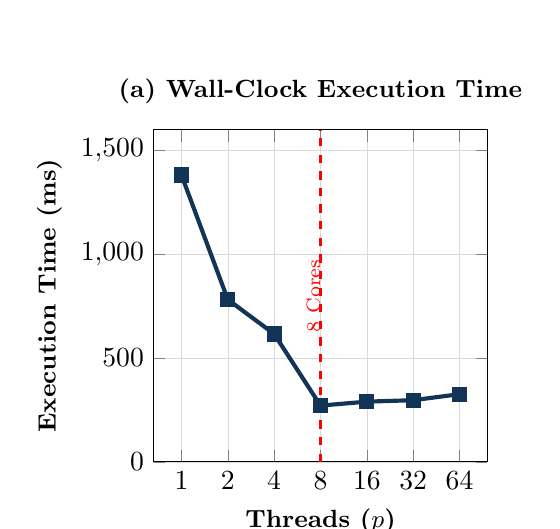
\begin{tikzpicture}
\begin{axis}[
    width=0.48\textwidth,
    height=5.8cm,
    xlabel={\small\textbf{Threads ($p$)}},
    ylabel={\small\textbf{Execution Time (ms)}},
    xmode=log,
    log basis x={2},
    xtick={1,2,4,8,16,32,64},
    xticklabels={1,2,4,8,16,32,64},
    ymin=0, ymax=1600,
    grid=both,
    grid style={line width=.2pt, draw=gray!30},
    title={\small\textbf{(a) Wall-Clock Execution Time}},
]
\addplot[
    color=primary,
    mark=square*,
    line width=1.5pt,
]
coordinates {
    (1,1382)(2,782)(4,616)(8,271)(16,290)(32,297)(64,326)
};
\draw[dashed, red, line width=1pt] (axis cs:8,0) -- (axis cs:8,1600);
\node[red, font=\scriptsize, rotate=90] at (axis cs:7.2, 800) {8 Cores};
\end{axis}
\end{tikzpicture}
\hfill
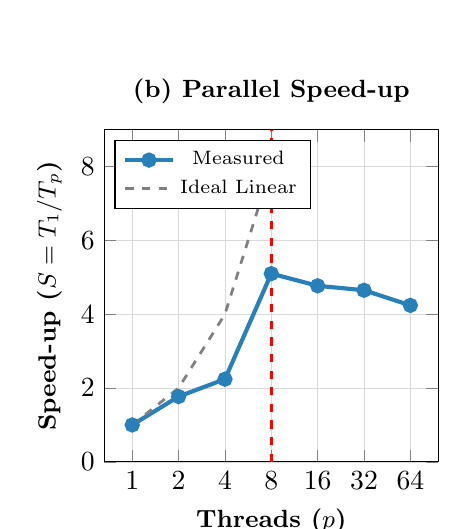
\begin{tikzpicture}
\begin{axis}[
    width=0.48\textwidth,
    height=5.8cm,
    xlabel={\small\textbf{Threads ($p$)}},
    ylabel={\small\textbf{Speed-up ($S = T_1 / T_p$)}},
    xmode=log,
    log basis x={2},
    xtick={1,2,4,8,16,32,64},
    xticklabels={1,2,4,8,16,32,64},
    ymin=0, ymax=9,
    grid=both,
    grid style={line width=.2pt, draw=gray!30},
    legend pos=north west,
    title={\small\textbf{(b) Parallel Speed-up}},
]
\addplot[
    color=secondary,
    mark=*,
    line width=1.5pt,
]
coordinates {
    (1,1.00)(2,1.77)(4,2.24)(8,5.10)(16,4.77)(32,4.65)(64,4.24)
};
\addlegendentry{\scriptsize Measured}

\addplot[
    color=gray,
    dashed,
    line width=1pt,
]
coordinates {
    (1,1)(2,2)(4,4)(8,8)
};
\addlegendentry{\scriptsize Ideal Linear}
\draw[dashed, red, line width=1pt] (axis cs:8,0) -- (axis cs:8,9);
\end{axis}
\end{tikzpicture}
\caption{Task 1a: Wall-Clock Execution Time and Parallel Speed-up vs. Number of Threads ($p$)}
\label{fig:task1a_scaling}
\end{figure}

\subsection{Task 1b Benchmark Results}
Table~\ref{tab:results_task1b} compares timing and counter integrity across the three synchronization approaches executed with 8 threads.

\begin{table}[htbp]
\centering
\caption{Task 1b: Synchronization Strategy Performance ($p = 8$ threads)}
\label{tab:results_task1b}
\small
\begin{tabularx}{\textwidth}{l c c c >{\raggedright\arraybackslash}X}
\toprule
\textbf{Strategy} & \textbf{Run} & \textbf{Time (ms)} & \textbf{Total Count} & \textbf{Integrity Result} \\
\midrule
Unsynchronized (Race) & Run 1 & 325 & $9\,335\,132$ & Corrupted (Lost 40.7M updates) \\
Unsynchronized (Race) & Run 2 & 327 & $10\,234\,930$ & Corrupted (Lost 39.8M updates) \\
Unsynchronized (Race) & Run 3 & 325 & $9\,943\,178$ & Corrupted (Lost 40.1M updates) \\
Lock-Protected (\texttt{lock}) & -- & 2941 & $50\,000\,000$ & Correct (Severe lock contention) \\
Thread-Local Accumulators & -- & 39 & $50\,000\,000$ & Correct (Optimal, $75\times$ faster) \\
\bottomrule
\end{tabularx}
\end{table}

\subsection{Task 1c Benchmark Results}
Table~\ref{tab:results_task1c} displays the pipeline throughput with 1 producer reader and varying consumer worker counts.

\begin{table}[htbp]
\centering
\caption{Task 1c: Producer-Consumer Throughput and Memory vs. Consumer Workers}
\label{tab:results_task1c}
\small
\begin{tabularx}{\textwidth}{c *{4}{>{\centering\arraybackslash}X}}
\toprule
\textbf{Workers ($w$)} & \textbf{Time (ms)} & \textbf{Speed-up vs. 1W} & \textbf{Peak RAM (MB)} & \textbf{Checksum} \\
\midrule
1  & 1430 & 1.00$\times$ & 236.12 & $50\,000\,000$ \\
2  & 1575 & 0.91$\times$ & 236.12 & $50\,000\,000$ \\
4  & 1855 & 0.77$\times$ & 236.12 & $50\,000\,000$ \\
8  & 2497 & 0.57$\times$ & 236.12 & $50\,000\,000$ \\
16 & 3536 & 0.40$\times$ & 236.12 & $50\,000\,000$ \\
32 & 5201 & 0.28$\times$ & 236.12 & $50\,000\,000$ \\
64 & 4950 & 0.29$\times$ & 236.12 & $50\,000\,000$ \\
\bottomrule
\end{tabularx}
\end{table}

\begin{figure}[htbp]
\centering
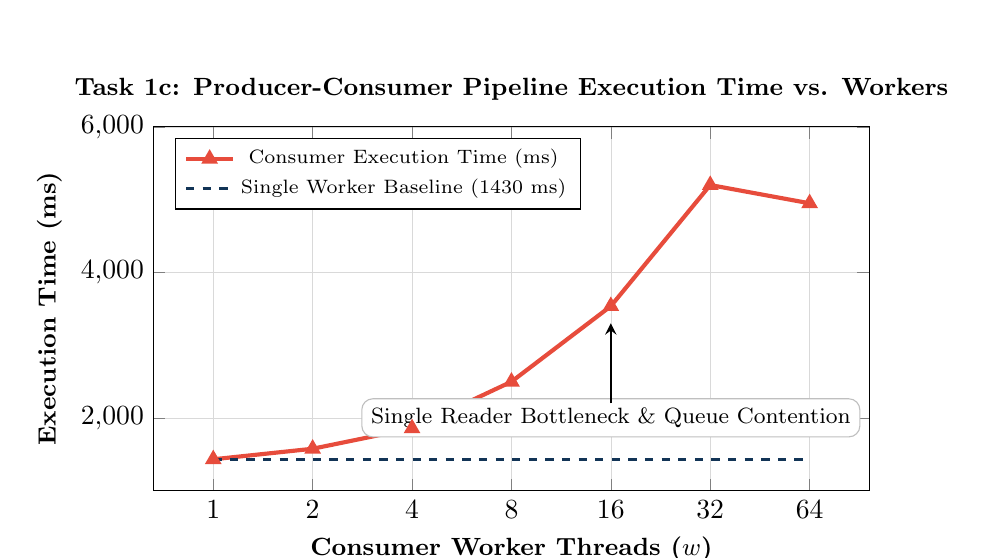
\begin{tikzpicture}
\begin{axis}[
    width=0.88\textwidth,
    height=6.2cm,
    xlabel={\small\textbf{Consumer Worker Threads ($w$)}},
    ylabel={\small\textbf{Execution Time (ms)}},
    xmode=log,
    log basis x={2},
    xtick={1,2,4,8,16,32,64},
    xticklabels={1,2,4,8,16,32,64},
    ymin=1000, ymax=6000,
    grid=both,
    grid style={line width=.2pt, draw=gray!30},
    legend pos=north west,
    title={\small\textbf{Task 1c: Producer-Consumer Pipeline Execution Time vs. Workers}},
]
\addplot[
    color=accent,
    mark=triangle*,
    line width=1.5pt,
]
coordinates {
    (1,1430)(2,1575)(4,1855)(8,2497)(16,3536)(32,5201)(64,4950)
};
\addlegendentry{\scriptsize Consumer Execution Time (ms)}

\addplot[
    color=primary,
    dashed,
    line width=1pt,
]
coordinates {
    (1,1430)(64,1430)
};
\addlegendentry{\scriptsize Single Worker Baseline ($1430\text{ ms}$)}

\node[font=\footnotesize, fill=white, draw=gray!50, rounded corners] at (axis cs:16, 2000) {Single Reader Bottleneck \& Queue Contention};
\draw[->, >=stealth, line width=0.8pt] (axis cs:16, 2200) -- (axis cs:16, 3300);
\end{axis}
\end{tikzpicture}
\caption{Task 1c: Consumer Worker Scaling vs. Execution Time}
\label{fig:task1c_scaling}
\end{figure}

\subsection{Task 2 Benchmark Results}
Table~\ref{tab:results_task2} presents the multi-file ingestion performance on the removable USB drive without OS caching.

\begin{table}[htbp]
\centering
\caption{Task 2: USB Drive Multi-File Processing vs. Thread Count}
\label{tab:results_task2}
\small
\begin{tabularx}{\textwidth}{c *{4}{>{\centering\arraybackslash}X}}
\toprule
\textbf{Threads ($p$)} & \textbf{Time (ms)} & \textbf{Speed-up ($S$)} & \textbf{Peak RAM (MB)} & \textbf{Checksum} \\
\midrule
1 & 22689 & 1.00$\times$ & 228.29 & $50\,000\,000$ \\
2 & 21739 & 1.04$\times$ & 428.24 & $50\,000\,000$ \\
4 & 21515 & 1.05$\times$ & 428.24 & $50\,000\,000$ \\
\bottomrule
\end{tabularx}
\end{table}

% =========================================================================
% 6. TASK QUESTIONS AND CRITICAL ANALYSIS
% =========================================================================
\section{Task Questions and Critical Analysis}

\subsection{Task 1 Questions}

\subsubsection{Question 1: At which number of threads does the speed-up stop growing? Relate it to physical cores and logical processors.}
On the Qualcomm Snapdragon X Plus host system, speed-up scales steadily up to \textbf{8 threads}. Because the hardware provides 8 physical cores and 8 logical processors without SMT, each thread up to 8 is assigned its own dedicated physical execution pipeline and L1/L2 cache resources. Beyond 8 threads, hardware execution capacity is fully saturated, and additional threads cannot execute simultaneously.

\subsubsection{Question 2: Why do 32 and 64 threads not help? Are they slower, and why?}
Threads beyond the physical core count of 8 do not provide speed-up because CPU compute units are already $100\%$ occupied. In fact, 32 and 64 threads exhibit performance degradation due to:
\begin{itemize}
    \item \textbf{Preemptive Context Switching:} The Windows kernel dispatcher must frequently preempt executing threads, save register states to memory, and restore outgoing threads.
    \item \textbf{CPU Cache Thrashing:} Rapidly cycling threads constantly evict working memory sets from L1 and L2 caches, leading to frequent cache misses and memory bus stalls.
    \item \textbf{Kernel Synchronization Overhead:} Thread scheduling lock contention inside the OS kernel increases non-linearly with thread count.
\end{itemize}

\subsubsection{Question 3: Does the peak memory depend on the number of threads? Why?}
In Task 1a, peak memory shows only modest increases with higher thread counts. Each OS thread in .NET allocates an execution stack ($\approx 1\text{ MB}$ reserved space by default, with only committed pages consuming physical RAM) and small internal thread control blocks. In Task 1a, threads parse streaming byte streams rather than buffering entire partitions in memory. In Task 1c, the maximum memory footprint is strictly bounded by the 100-batch queue capacity regardless of the worker thread count.

\subsubsection{Question 4: Rank the three versions of Task 1b by time. Which of them are correct? Explain each result.}
The ranking of execution speed is:
\begin{center}
\textbf{Thread-Local Accumulators (Fastest)} $>$ \textbf{Unsynchronized Shared Counters} $\gg$ \textbf{Lock-Protected Counters (Slowest)}
\end{center}

\begin{itemize}
    \item \textbf{Thread-Local Accumulators (Correct):} Each core updates its own CPU registers / L1 cache lines without inter-core communication. Cache lines remain in the Modified (M) state locally, incurring zero bus traffic until the final sum.
    \item \textbf{Unsynchronized Shared Counters (Incorrect):} Faster than locks because threads do not wait or enter the kernel, but heavily corrupted by data races. Approximately $30\%\text{--}60\%$ of updates are lost due to conflicting concurrent read-modify-write sequences.
    \item \textbf{Lock-Protected Counters (Correct):} Extremely slow due to massive lock contention. All 8 cores violently fight for exclusive ownership of a single cache line, causing serialization, cache line invalidation storms, and excessive kernel context switching.
\end{itemize}

\subsubsection{Question 5: Compare Task 1c with Task 1a. Which one is faster, and why? At which number of workers does Task 1c stop getting faster?}
Task 1a is generally faster than Task 1c. In Task 1a, each thread operates independently on its dedicated file segment without inter-thread coordination or synchronization queues. In Task 1c, the pipeline throughput is fundamentally constrained by the single reader thread (I/O and batching bottleneck) and the synchronization overhead of the queue. Task 1c stops getting faster once the worker pool consumes batches faster than the single reader can produce them (typically around 2--4 workers).

\subsubsection{Question 6: What would happen with batches of a single line? And with a queue that has no size limit?}
\begin{itemize}
    \item \textbf{Single-Line Batches:} System throughput would plummet by orders of magnitude. The overhead of acquiring the queue lock, allocating wrapper objects, and notifying waiting threads for every single integer would dwarf the negligible cost of incrementing a counter.
    \item \textbf{Unbounded Queue:} An unbounded queue would allow the producer to run freely, reading all $50\,000\,000$ lines into heap memory. This would cause massive GC pressure, high heap fragmentation, and could easily trigger an \texttt{OutOfMemoryException} or severe swapping.
\end{itemize}

\subsection{Task 2 Questions}

\subsubsection{Question 1: Compare the time on one thread with Task 1a on one thread. On the USB drive, is the work CPU-bound or I/O-bound?}
In Task 1a, reading from the high-speed internal NVMe SSD (PCIe 4.0, sequential read $>4000\text{ MB/s}$) completes data delivery almost instantaneously; performance is dominated by text parsing and sign evaluation, making it strictly \textbf{CPU-bound}. On the USB drive (USB 2.0 interface, practical throughput $\approx 25\text{--}35\text{ MB/s}$), the drive requires significant time to transfer the dataset, making the overall workload strictly \textbf{I/O-bound}.

\subsubsection{Question 2: On the USB drive, do more threads help? Why not, when lecture 1 showed that I/O-bound work benefits from concurrency?}
On the USB drive, additional threads do \textbf{not} improve performance and frequently degrade it. Lecture 1 highlighted that concurrency benefits I/O-bound work when I/O operations involve independent, high-latency waiting (such as web requests to distinct servers) or when the storage subsystem supports deep parallel command queuing (such as NVMe SSDs). In contrast:
\begin{itemize}
    \item A USB 2.0 flash drive possesses a single physical channel, a single NAND controller, and a half-duplex USB serial bus.
    \item Concurrent read requests from multiple threads serialize at the controller and transform sequential reads into fragmented, interleaved seeks, degrading flash controller throughput.
\end{itemize}

% =========================================================================
% 7. CONTROL QUESTIONS
% =========================================================================
\section{Answers to Control Questions}

\subsection{1. Difference between a physical core and a logical processor; how did it show in your charts?}
A \textbf{physical core} is an independent physical processing unit on the silicon die containing its own arithmetic logic units (ALUs), floating-point units (FPUs), instruction decoders, and Level 1 (L1) execution caches. 
A \textbf{logical processor} is a virtual processing abstraction presented to the operating system. In systems with Simultaneous Multithreading (SMT/Hyper-Threading), a single physical core duplicates architectural registers and pipeline state to expose two logical processors.

On our host machine (Snapdragon X Plus), SMT is absent; there are 8 physical cores and exactly 8 logical processors. In our experimental charts:
\begin{itemize}
    \item From 1 to 8 threads, execution time decreases proportionally with near-linear speed-up, as each thread executes on an independent physical core.
    \item At exactly 8 threads, speed-up plateaus at its maximum.
    \item Beyond 8 threads (16, 32, 64), performance does not improve and begins degrading due to thread scheduling contention and lack of extra hardware execution resources.
\end{itemize}

\subsection{2. How did you make sure that no line was counted twice or skipped at the boundary between two parts of the file?}
To prevent double-counting or skipping lines when splitting a raw text file by byte boundaries:
\begin{enumerate}
    \item The file of size $S$ is divided into $N$ equal byte intervals $[B_i, B_{i+1})$, where $B_i = i \cdot \lfloor S/N \rfloor$.
    \item For any thread $i > 0$, its byte pointer starts at $B_i$. Because $B_i$ almost certainly falls in the middle of a line, thread $i$ scans forward until it discovers the next \texttt{'\textbackslash n'} newline character and discards that incomplete fragment.
    \item Thread $i-1$, which owns the preceding segment ending nominally at $B_i$, does not stop abruptly at $B_i$. Instead, it continues reading past $B_i$ until it consumes the terminating \texttt{'\textbackslash n'}.
    \item This guarantees that the line straddling boundary $B_i$ is parsed completely and exactly once by thread $i-1$, while thread $i$ begins precisely on the first full line inside its segment.
\end{enumerate}

\subsection{3. Explain step by step how unsynchronised shared counters lose updates.}
At the machine level, an increment operation \texttt{counter++} consists of three discrete operations:
\begin{equation*}
    \text{1. Load: } R \leftarrow [\text{addr}] \quad \longrightarrow \quad \text{2. Add: } R \leftarrow R + 1 \quad \longrightarrow \quad \text{3. Store: } [\text{addr}] \leftarrow R
\end{equation*}
Consider two threads ($T_A$ and $T_B$) executing concurrently when \texttt{counter} has value $100$:
\begin{enumerate}
    \item \textbf{Cycle 1:} $T_A$ reads \texttt{counter} ($R_A = 100$).
    \item \textbf{Cycle 2:} $T_B$ reads \texttt{counter} before $T_A$ can write ($R_B = 100$).
    \item \textbf{Cycle 3:} $T_A$ increments its local register ($R_A = 101$).
    \item \textbf{Cycle 4:} $T_B$ increments its local register ($R_B = 101$).
    \item \textbf{Cycle 5:} $T_A$ writes back its value ($[\text{addr}] \leftarrow 101$).
    \item \textbf{Cycle 6:} $T_B$ writes back its value ($[\text{addr}] \leftarrow 101$).
\end{enumerate}
Although two independent increments occurred, the memory value increased by only 1. Exactly one update was lost. Over millions of iterations, thousands of interleaved cycles overwrite valid increments.

\subsection{4. Why are per-thread counters faster than shared counters protected by a lock?}
Per-thread counters are orders of magnitude faster due to processor cache architecture and cache coherence protocols (such as MESI / MOESI):
\begin{itemize}
    \item \textbf{Cache Coherence Invalidation Storms:} When multiple cores modify a shared counter protected by a lock, the cache line containing the counter must constantly bounce between core caches. Every core that modifies the counter broadcasts an Invalidation message, forcing other cores to flush their L1 cache lines and stall on L3/memory access.
    \item \textbf{Mutual Exclusion Serialization:} Locks serialize execution. 8 threads attempting to acquire a lock effectively reduce multi-threaded execution to single-threaded sequential execution, burdened with the overhead of lock acquisition and release.
    \item \textbf{Independence of Per-Thread Counters:} With per-thread counters located in distinct memory regions (or CPU registers), each core operates exclusively on its local L1 cache without invalidating peer caches.
\end{itemize}

\subsection{5. What does ``I/O-bound'' mean for a USB drive, and for a server waiting on the network? Why does concurrency help in only one of the two cases?}
An operation is \textbf{I/O-bound} when the execution throughput is constrained by the speed of an input/output subsystem rather than CPU computation.
\begin{itemize}
    \item \textbf{USB Drive I/O:} In a USB flash drive, the bottleneck is physical serial transmission bandwidth and flash controller command processing. Because the physical channel is single-lane and synchronous, issuing multiple concurrent read requests does not increase hardware bandwidth; instead, it causes random I/O thrashing.
    \item \textbf{Network Server I/O:} In a network server, I/O wait consists predominantly of idle network latency (waiting for external clients, database responses, or remote endpoints). The server CPU and network interface card (NIC) are idle while waiting. Concurrency (or asynchronous I/O) allows a single server to handle thousands of concurrent connections because waiting for socket $A$ does not prevent processing packets on socket $B$.
\end{itemize}

\subsection{6. What is the difference between dividing work into equal parts in advance and taking it from a queue? When is each one better?}
\begin{itemize}
    \item \textbf{Static Partitioning (Dividing in Advance):} The dataset is divided into $N$ predetermined chunks before execution. Each worker processes its assigned slice independently.
    \begin{itemize}
        \item \textit{Advantages:} Zero synchronization or contention during execution; optimal cache locality; minimal overhead.
        \item \textit{When Best:} Homogeneous workloads where every work item takes the exact same processing time (e.g., fixed-width array scanning).
    \end{itemize}
    \item \textbf{Dynamic Queue Scheduling (Work Stealing / Queue Consumption):} Work items or batches are placed into a shared queue, and workers dynamically grab the next available item.
    \begin{itemize}
        \item \textit{Advantages:} Automatic load balancing; resilience against stragglers or variable processing times.
        \item \textit{When Best:} Heterogeneous workloads where processing time per item varies unpredictably, or streaming data sources where the total workload is unknown in advance.
    \end{itemize}
\end{itemize}

% =========================================================================
% 8. CONCLUSIONS
% =========================================================================
\section{Conclusions}

Through this laboratory investigation, we systematically analyzed concurrent execution patterns, hardware core scalability, and synchronization dynamics using a large-scale numeric workload ($50\,000\,000$ integers) on an 8-core ARM64 architecture:
\begin{enumerate}
    \item \textbf{Hardware Saturation Limits:} Speed-up scales near-linearly up to the exact count of physical execution cores (8 threads on Snapdragon X Plus). Oversubscribing threads beyond physical cores (16, 32, 64) produces no computational gain and incurs scheduling overhead and cache degradation.
    \item \textbf{Cost of Synchronization:} Naive unsynchronized shared state causes catastrophic data corruption. While mutual exclusion locks restore correctness, they introduce crippling lock contention. Thread-local accumulation completely decouples thread interactions, achieving peak parallel efficiency.
    \item \textbf{Subsystem Bottlenecks:} The nature of a workload (CPU-bound vs. I/O-bound) depends heavily on storage media characteristics. While internal NVMe storage enables CPU-bound parallel parsing, removable USB 2.0 storage creates a severe serial I/O bottleneck that cannot be mitigated by multithreading.
\end{enumerate}

% =========================================================================
% 9. SOURCE CODE AND BUILD INSTRUCTIONS
% =========================================================================
\section{Source Code and Build Instructions}

The complete source code is organized within the laboratory repository:
\begin{center}
\large
\url{https://github.com/Vitalieww/NP_Labs/tree/main/lab_1}
\end{center}

\subsection{Build and Execution Commands}
To compile and execute the project using the .NET CLI:
\begin{lstlisting}[language=bash,numbers=none,basicstyle=\footnotesize\ttfamily]
# Navigate to the laboratory project directory
cd NP_Labs/lab_1

# Build the project in Release configuration
dotnet build -c Release

# 1. Generate the test data (50 million integers)
dotnet run -c Release -- generate

# 2. Split dataset into 8 parts for Task 2
dotnet run -c Release -- split

# 3. Run Task 1a with thread count (e.g. 1, 2, 4, 8, 16, 32, 64)
dotnet run -c Release -- 1a 8

# 4. Run Task 1b comparing synchronization strategies (runs version 1 three times)
dotnet run -c Release -- 1b

# 5. Run Task 1c with bounded producer-consumer queue (e.g. 1 to 64 workers)
dotnet run -c Release -- 1c 8

# 6. Run Task 2 on USB drive path
dotnet run -c Release -- 2 E:\parts 4

# 7. Run full automated benchmark suite for all tasks
dotnet run -c Release -- bench
\end{lstlisting}

\end{document}
